\begin{appendices}
%\addappheadtotoc

\chapter{Intrabundle Usage}

\section{Setup environment}

In this work we provide a customized Forge distribution. This distribution downloads Intrabundle from its source code repository and automatically installs it in Forge environment when Forge is started.

The only prerequisite is to have JAVA\_HOME environment system variable pointing to a Java 6 or higher installation. Below are the steps to install Intrabundle and Forge:


\begin{enumerate}
\item Download Intrabundle Forge distribution from sourceforge: \\ \href{http://sourceforge.net/projects/intrabundle/files/latest/download}{http://sourceforge.net/projects/intrabundle/files/latest/download};
\item unzip it to a folder, i will call it HOME in this tutorial;
\item execute \emph{HOME/bin/forge} file if you are on Linux or MacOS, \\on Windows execute  \emph{HOME\textbackslash{}bin\textbackslash{}forge.bat} file;
\item you should see image \ref{forge start} and image \ref{intrabundle installation} as below:
\begin{figure}[h]
\caption{Forge start}
\label{forge start}
\centering
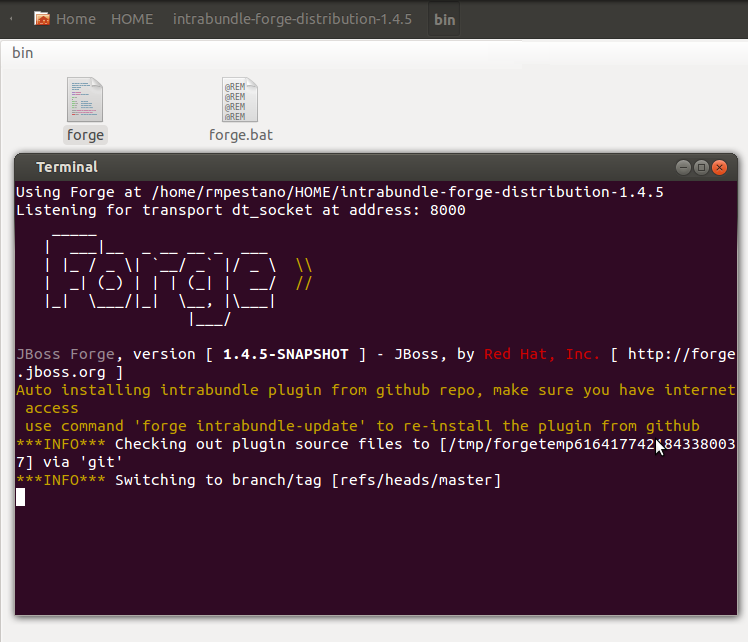
\includegraphics[scale=0.5]{tutorial01}
\end{figure}
\FloatBarrier

Intrabundle should be installed from its online source code repository, make sure you have internet access during this process:

\begin{figure}[h]
\caption{Intrabundle installation}
\label{intrabundle installation}
\centering
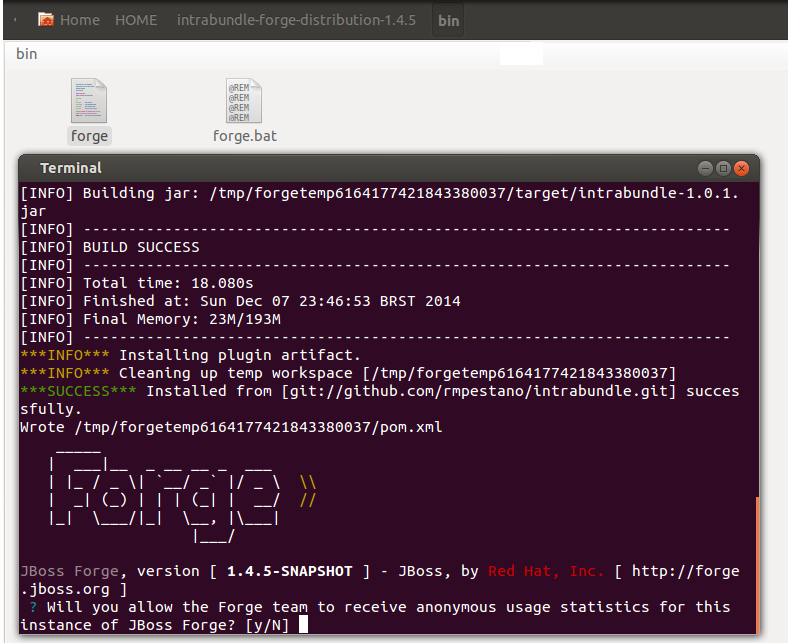
\includegraphics[scale=0.5]{tutorial02}
\end{figure}
\FloatBarrier
\end{enumerate}

There is also an online video you can watch to get you started with Intrabundle, see \citep{intrabundle github 2014}.

From now on you are ready to fire Forge and Intrabundle commands. 

\section{Begin Introspection}
With Forge up and running now you can start OSGi project introspection with Intrabundle. An example OSGi project can be found at \\
 \href{http://www.dcc.ufmg.br/\textasciitilde{}mtov/osgi\_example.zip}{http://www.dcc.ufmg.br/\textasciitilde{}mtov/osgi\_example.zip}, it is from the article \citep{Tavares 2008}.
Unzip the downloaded project to HOME and go back to Forge console.

Navigate to folder OSGI using \emph{cd} command: \emph{cd /HOME/OSGI}(you can use \emph{tab} for auto completion), like in Image \ref{navigate project}:

\begin{figure}[h]
\caption{Navigating to project}
\label{navigate project}
\centering
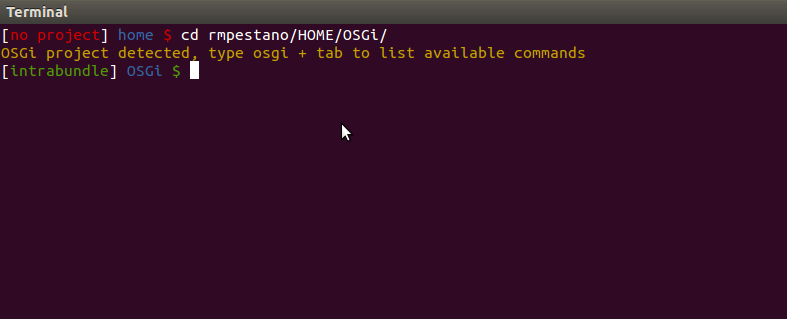
\includegraphics[scale=0.5]{tutorial03}
\end{figure}
\FloatBarrier
 
You can see that intrabundle recognized the OSGi project, so you can fire commands at OSGi project level like generate report or list bundles as well inspect its bundles, as in Image \ref{fire commands}:

\begin{figure}[h]
\caption{Fire commands}
\label{fire commands}
\centering
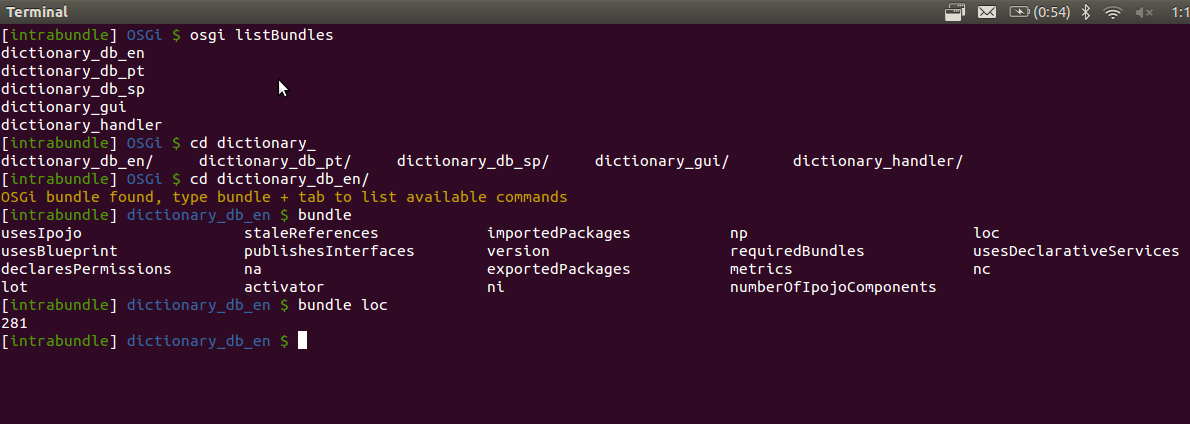
\includegraphics[scale=0.5]{tutorial04}
\end{figure}
\FloatBarrier

Another useful command Intrabundle provides is \emph{osgi-scan}, it search for OSGi bundles in file system and generate reports on top of them. To use it go back to HOME folder and fire \textbf{osgi-scan 2} command\footnote{number argument is the depth of folders to scan}, it must find bundles within downloaded project as is Image \ref{osgi-scan}:

\begin{figure}[h]
\caption{osgi-scan}
\label{osgi-scan}
\centering
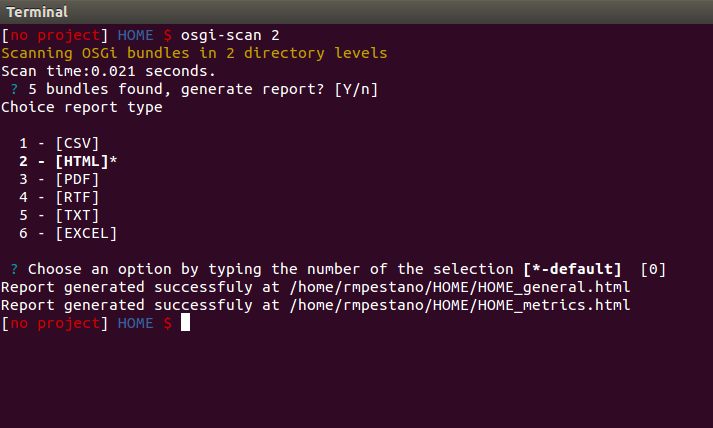
\includegraphics[scale=0.5]{tutorial05}
\end{figure}
\FloatBarrier
\end{appendices}
